\documentclass[12pt, a4paper, reqno]{article}
\usepackage[utf8]{inputenc}
\usepackage{amsmath, amsfonts, amssymb, amsthm, graphicx}
\usepackage[ruled]{algorithm2e}
\usepackage{caption}

\usepackage{hyperref}
\usepackage[dvipsnames]{xcolor}
\hypersetup{colorlinks, linkcolor={MidnightBlue}, citecolor={MidnightBlue}, urlcolor={MidnightBlue}} 

\usepackage{tikz}

\setlength{\parindent}{0pt}
\newcommand{\forceindent}{\leavevmode{\parindent=1em\indent}}
\numberwithin{equation}{section}
\addtolength{\textwidth}{2 truecm}
\setlength{\hoffset}{-1 truecm}

\newtheorem*{theorem*}{Theorem}
\newtheorem*{cor*}{Corollary}

\newcommand{\norm}[1]{\left\lVert#1\right\rVert}
\newcommand{\e}{\epsilon}
\newcommand{\w}{\omega}
\newcommand{\R}{\mathbb{R}}
\newcommand{\N}{\mathbb{N}}
\newcommand{\Q}{\mathbb{Q}}
\newcommand{\Z}{\mathbb{Z}}
\renewcommand{\ae}[1]{\text{ \hspace{5pt} a.e. #1}}

\begin{document}

\title{Combining $l^1$ Penalization with Higher Moment Feasible Sets in Regression Models: a STAT8053 Project}
\author{Austin David Brown}
\date{\today}
\maketitle


TOOD library may crash by design

TODO talk about convergence guarantee

\section{Introduction}

In statistics and probability theory it is common to impose moment assumptions on a random variable $X : \Omega \to \R^n$ such as $E(\norm{X}^k) < \infty$ for $k \in \R$.
These constraints correspond to the $L^p$ spaces which allow control over the width and the height of such random variables.
This can be interpreted as imposing "stability" on the random variable $X$.
If statisticians so freely impose such constraints then we should build a tool to allow scientists and researchers to impose such constraints on their real problems.
In this project, we build a package implements this idea.
The goal is not to create the best predicting method, but instead build a tool that will allow researchers to explore stability and what a "stable" solution to their problem may look like.

\forceindent I was genuinely curious as to what happens if the Elasticnet from Zou and Hastie \cite{elasticnet} had higher moments.
For simplicity, we consider exactly this with the penalty
\[
P(\lambda) = \lambda \alpha_1 \norm{\beta}_1 + \lambda \sum_{k = 1}^{5} \alpha_k \norm{\beta}_{2k}^{2k} 
\]
with $\sum_{k = 1}^{10} \alpha_k = 1$ and $10$ is chosen for no special reason.
This has a geometric interpretation.
Consider a particular Elasticnet penalty 
\[
1/2 |x| + 1/2 |y| + 1/2|x|^2 + 1/2|y|^2
\]
 shown on the left and a new penalization 
 \[
 1/2|x| + 1/2|y| + 1/2|x|^4 + 1/2|y|^4
 \] shown on the right.
It seems reasonable that a scientist or researcher may want to "bow" out the feasable set in a geometric sense.

\begin{center}
\begin{minipage}{.5\textwidth}
  \centering
  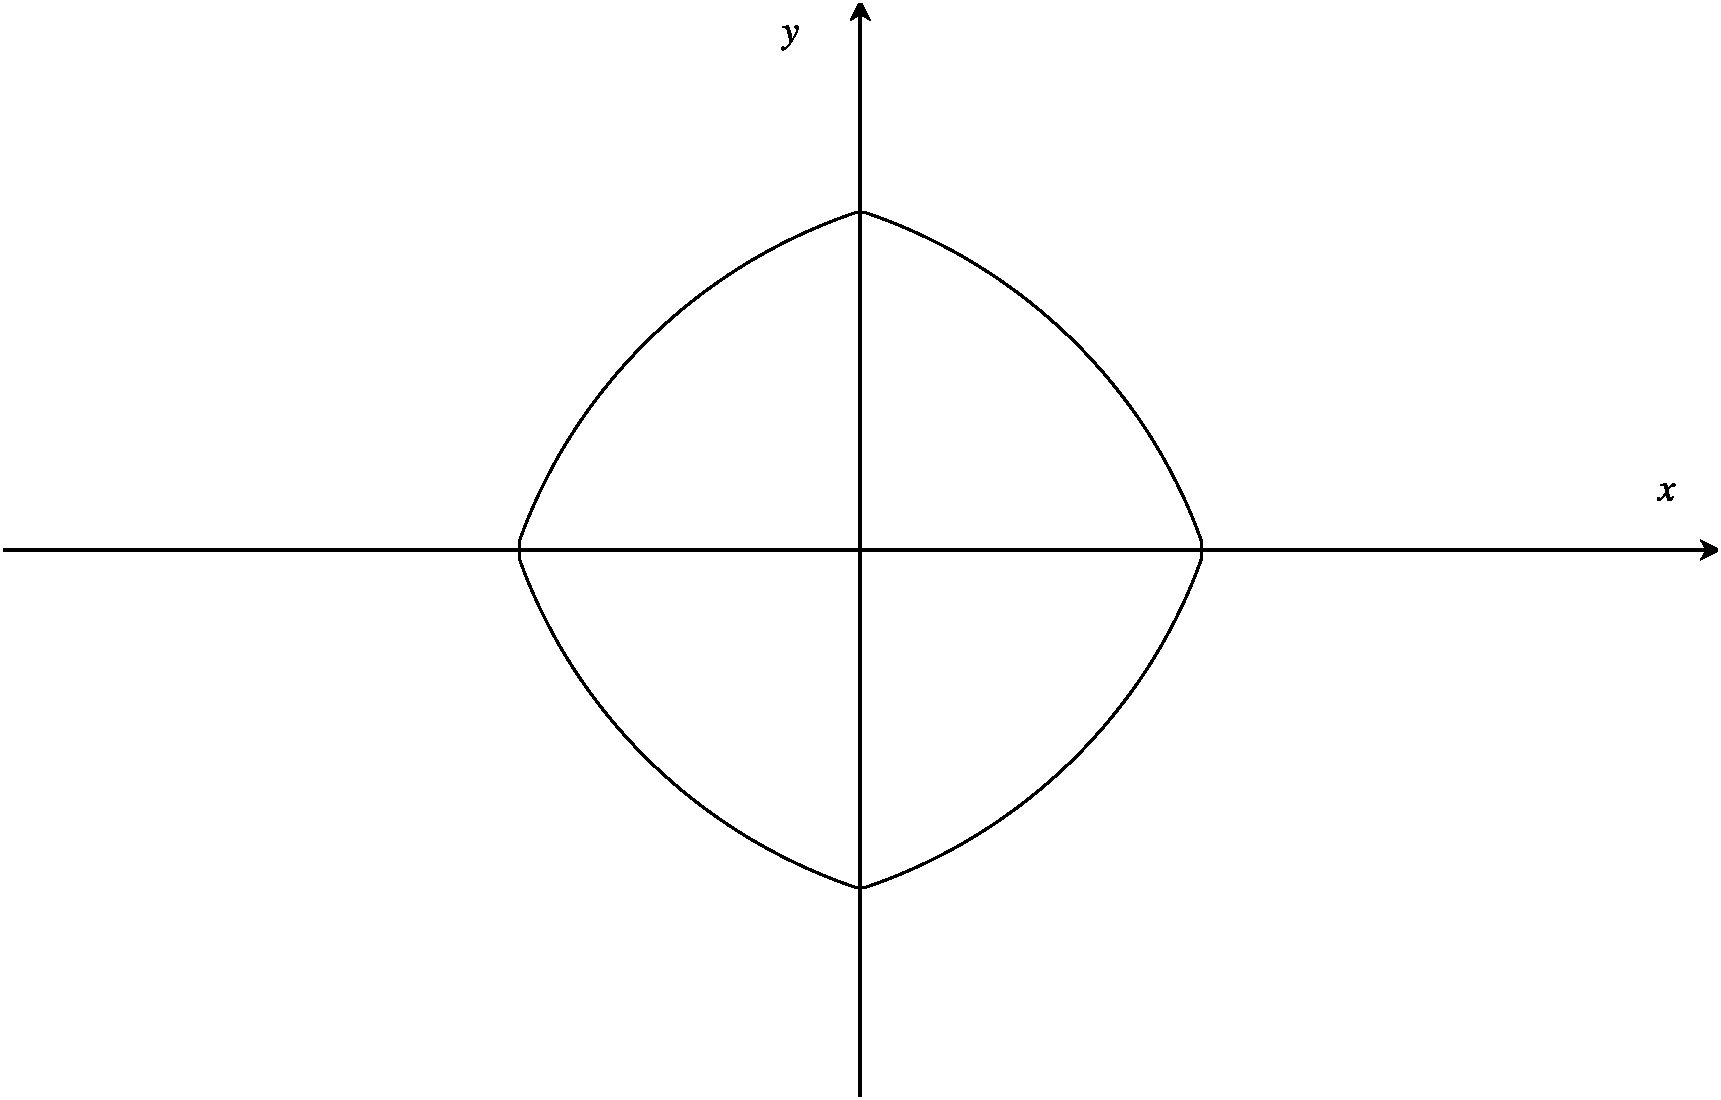
\includegraphics[width=.9\linewidth]{elasticnet.pdf}
\end{minipage}%
\begin{minipage}{.5\textwidth}
  \centering
  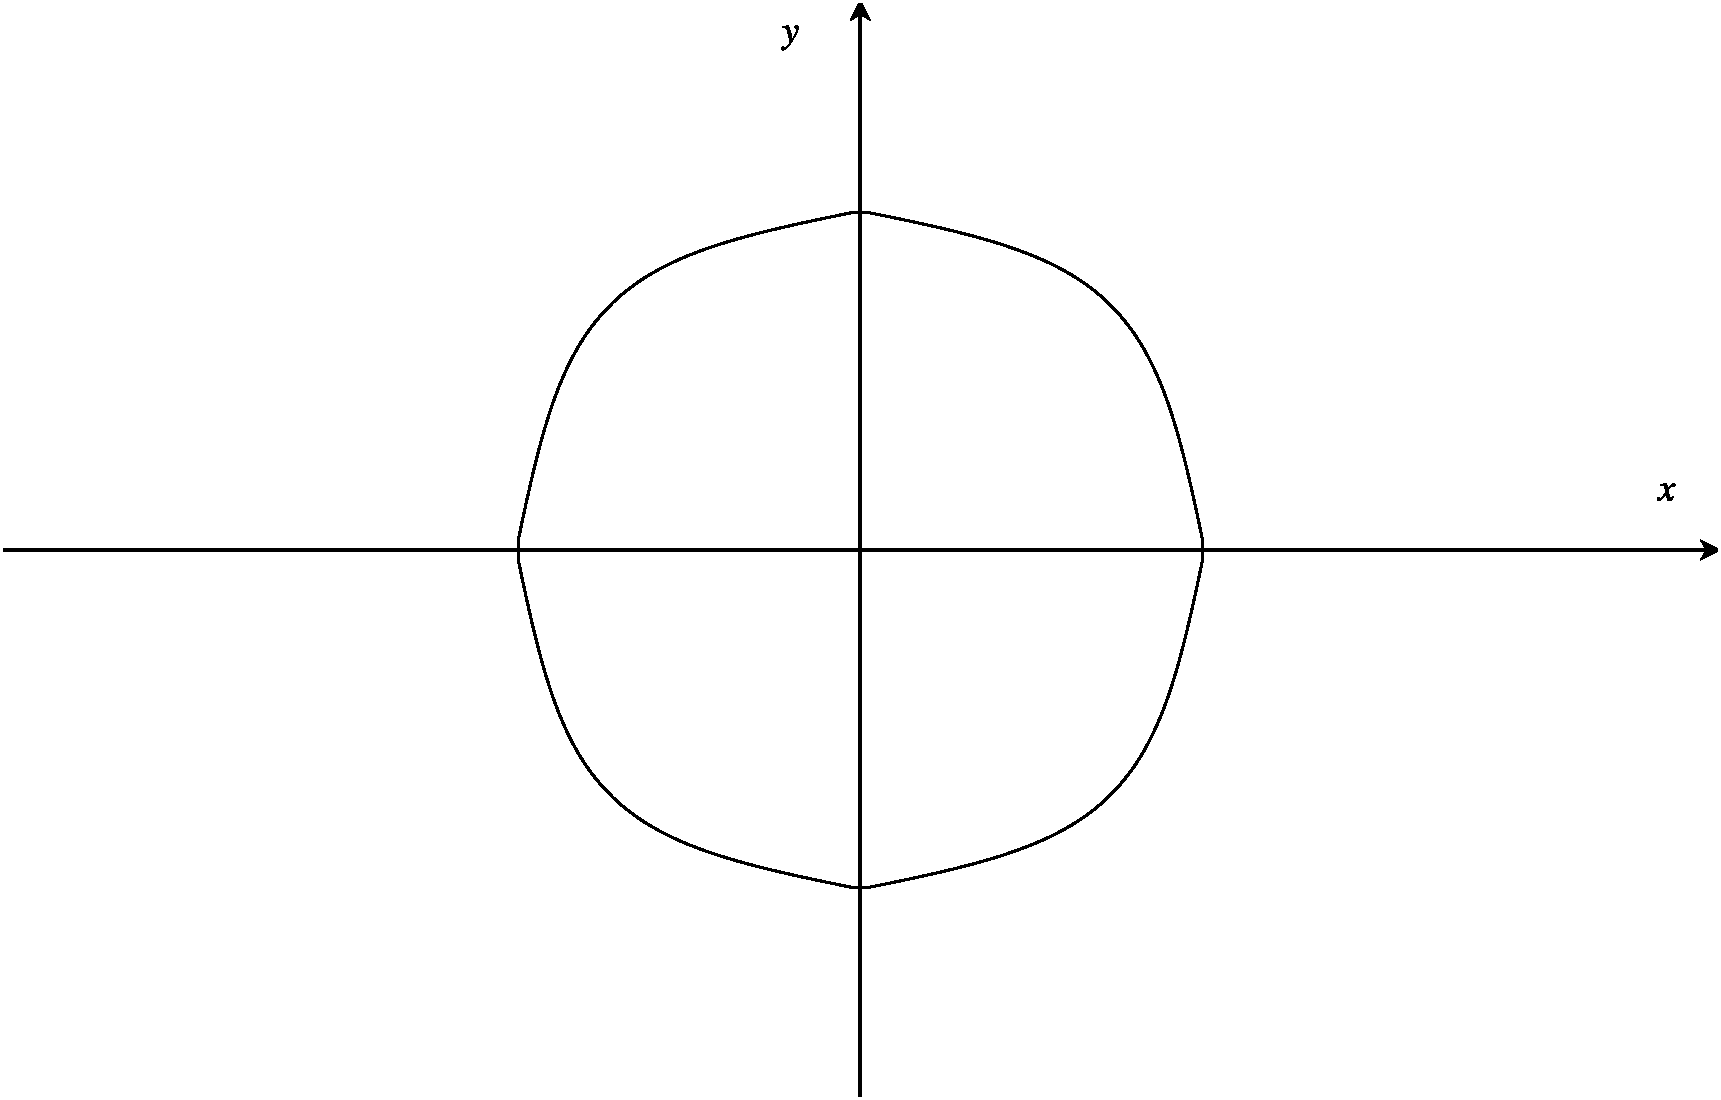
\includegraphics[width=.9\linewidth]{new_penalty_4_moment.pdf}
\end{minipage}
\captionof{figure}{A particular ElasticNet penalty shown on the left and a new penalty shown on the right shown to "bow" out the feasible set.}
\end{center}

Alternatively, the researcher wants to impose "stability" into their solutions by restricting the feasible set.
This is analagous to moment conditions in some sense since the researcher wants to control the sparsity along with the height and width of their solution.

\forceindent Another penalty I would like to explore in the future is combining the  $\norm{\cdot}_1$ and $\norm{\cdot}_\infty$ as
\[
P'(\lambda) = \lambda \alpha_1 \norm{\beta}_1 + \lambda \alpha_2 \norm{\beta}_\infty 
\]
This is be shown in the figure below.

\begin{center}
\begin{minipage}{.5\textwidth}
  \centering
  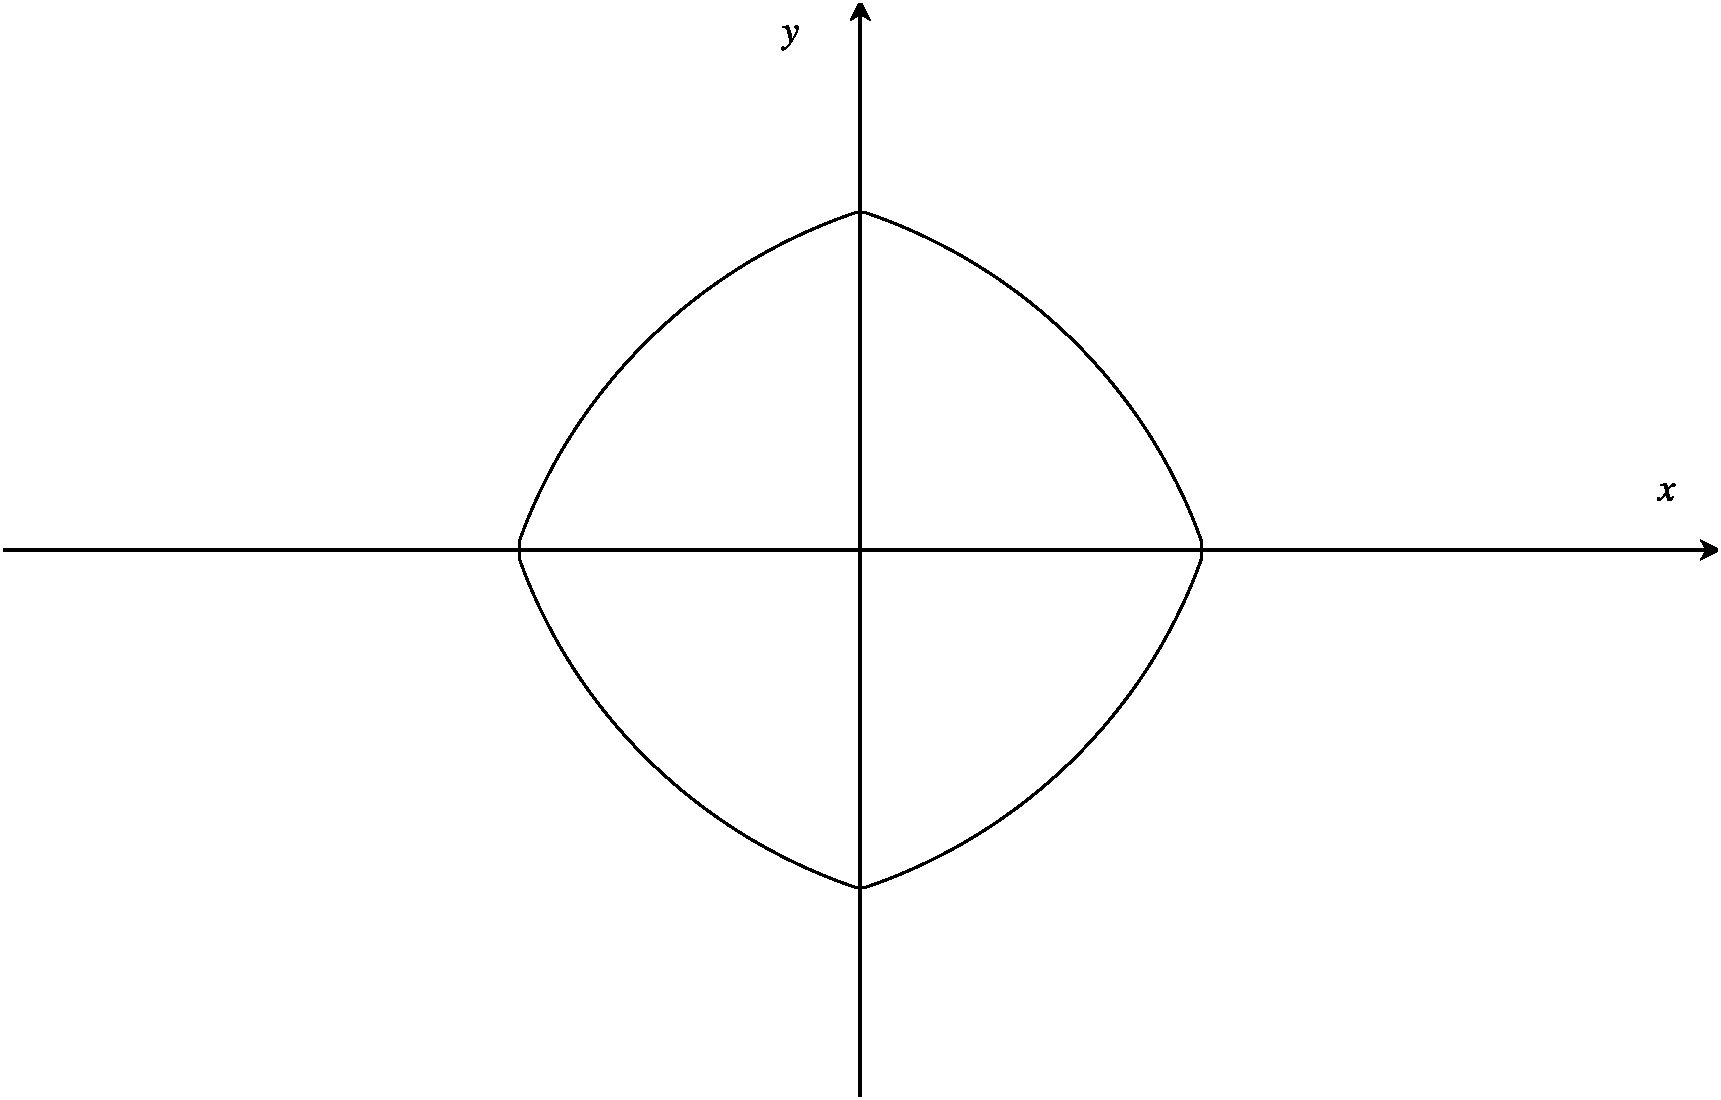
\includegraphics[width=.9\linewidth]{elasticnet.pdf}
\end{minipage}%
\begin{minipage}{.5\textwidth}
  \centering
  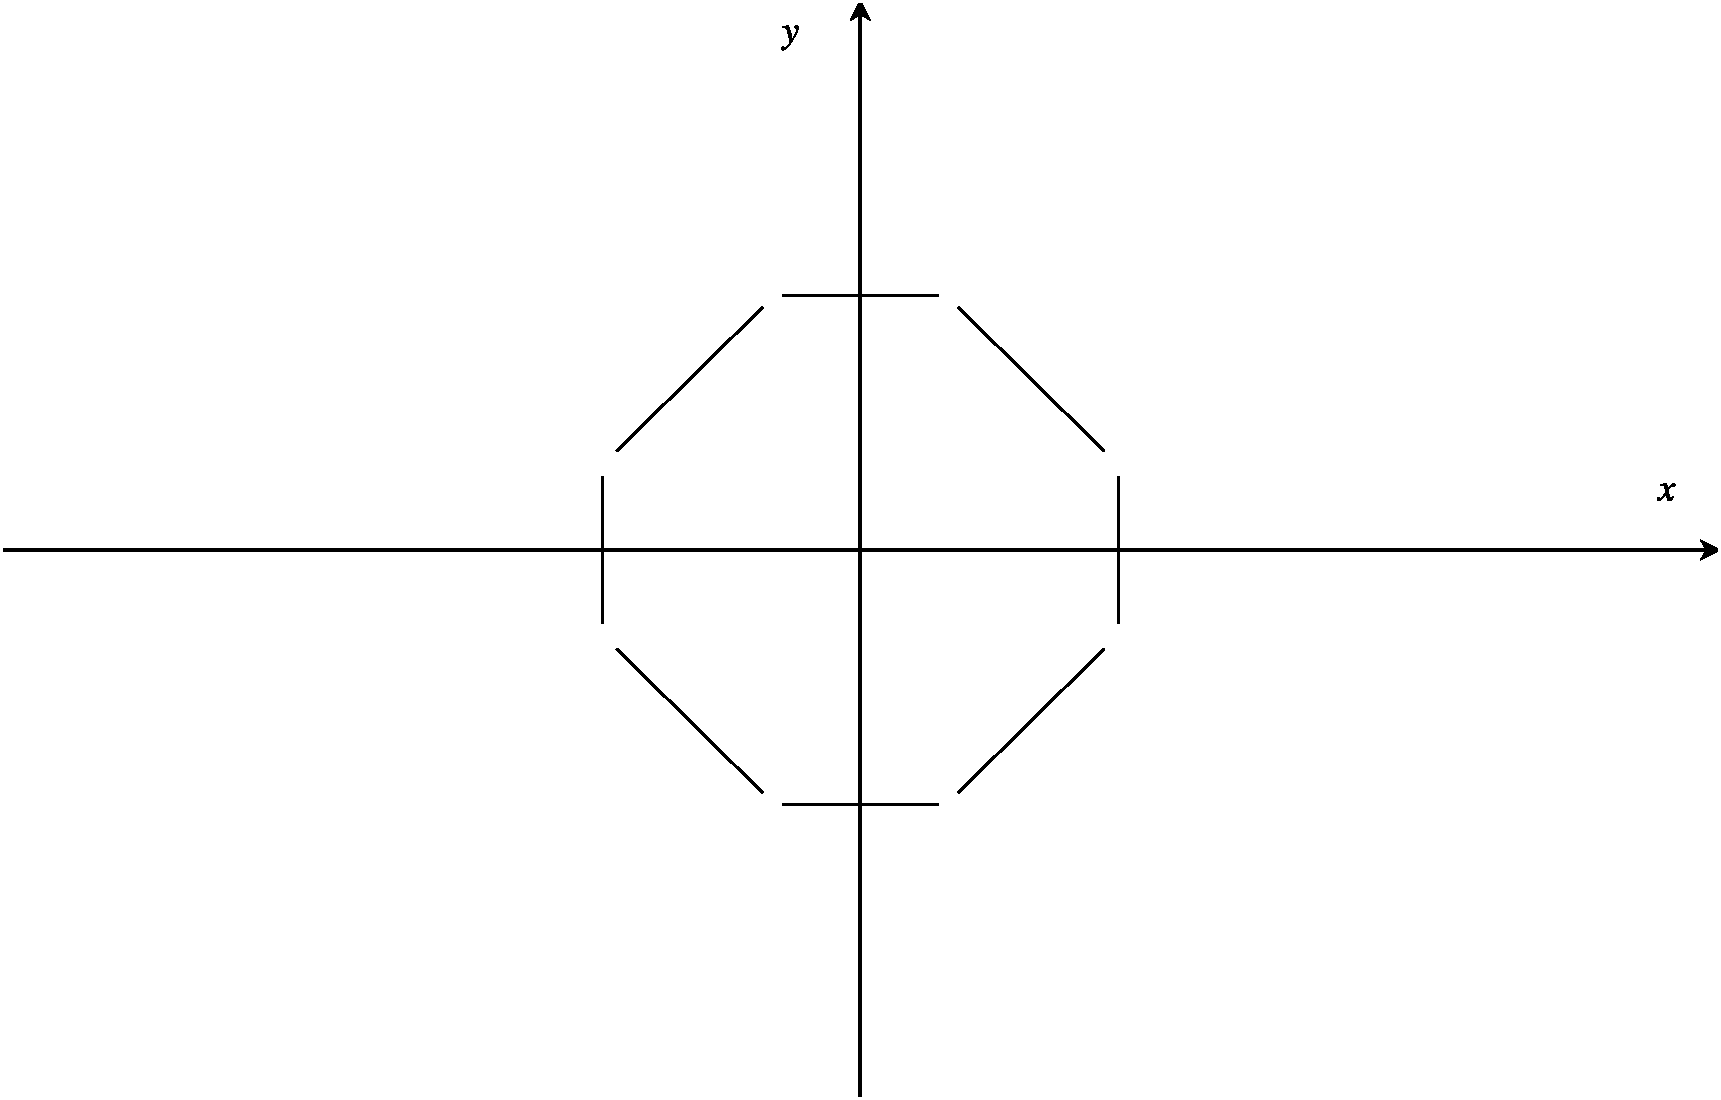
\includegraphics[width=.9\linewidth]{new_penalty_l1_and_linf.pdf}
\end{minipage}
\captionof{figure}{Elasticnet on the left and l1 and infinity norm on the right}
\end{center}

I believe this can be solved with the ADMM algorithm, but I ran out of time.




\section{Implementation}


In this section, we discuss how the package was implemented.
In the glmnet paper \cite{glmnet}, Friedman, Hastie and Tibshirani use coordinate descent.
With the elasticnet \cite{elasticnet} penalty, the coordinate wise minimization yields an analytic, closed form solution and line search or step size rules are not needed. With the penalty that we propose
\[
P(\lambda) = \lambda \alpha_1 \norm{\beta}_1 + \lambda \sum_{k = 1}^{5} \alpha_k \norm{\beta}_{2k}^{2k} 
\]
will not have an analytic solution and a new algorithm is needed.
This penalization also not Lipschitz continuous and makes convergence analysis more difficult.
An important point is that the $l^1$ penalty is not differentiable, but it is separable and so is this penalty and so coordinate-wise optimization will hold.
Let 
\[
L(\beta) = \frac{1}{2} \norm{y - X \beta}_2^2 + \lambda P(\beta)
\]
be the objective with $y \in \R^n$, $X \in M_{n \times p}(\R)$ centered, and $\beta \in \R^p$.
The first algorithm used for this problem was the subgradient coordinate method shown below.

\vspace{.5cm}
\begin{algorithm}[H]
\caption{Subgradient Coordinate Method}
Choose $\beta^0 \in \R^p$ and tolerance $\delta > 0$;

Set $k \gets 0$

\Repeat{Until the loss difference $\Delta L$ is less than $\delta$}{ 

  Set the step size $h^k \gets \frac{R}{\sqrt{1 + k}}$ for some $R > 0$ or use a constant step size.

  Permute $I = \{1, \ldots, p\}$

  \For {$i \in I$}{

    $\beta^{k + 1}_i \gets \beta^{k}_i - h^i g^i$ where $g^i \in (\partial L)_i$

  }

  $k \gets k + 1$
}

\end{algorithm}
\vspace{.5cm}

This algorithm is not a descent method, there is no good stopping criterion, and the non-differentiability is problematic to line search.
The diminishing step size was chosen due to Nesterov's analysis in \cite{nesterov}.
The stopping criterion is also expensive at $O(n^2)$ flops.
In our implementation, we experiences solutions without sparsity, but instead with very small values, so a thresholding function is needed to produce sparsity.


A better algorithm we discovered later was proximal gradient coordinate descent shown below.

\vspace{.5cm}
\begin{algorithm}[H]
\caption{Proximal Gradient Coordinate Descent}
Choose $\beta^0 \in \R^p$ and tolerance $\delta > 0$;

Set $k \gets 0$

\Repeat{Until the Moreau-Yoshida mapping $M_{h_k, f} < \delta$}{ 

  Set the step size $h^k > 0$ with diminishing or line search.

  Randomly permute $I = \{1, \ldots, p\}$

  \For {$i \in I$}{

    $\beta^{k + 1}_i \gets (\textbf{prox}_{h^k L})_i ( \beta^k_i - h^k \langle X_i, y - X \beta \rangle )$

  }

  $k \gets k + 1$
}
\end{algorithm}
\vspace{.5cm}

An important point is because the objective and penalization are separable, the proximal mapping is
\[
\textbf{prox}_{L}(x) = \left( \textbf{prox}_{L}(x_i))_i \right). 
\]
This is a descent method, line search can be done, and the stopping criterion is cheap to compute at $O(p^2)$.
Further, the convergence theory is the same as coordinate descent due to the Moreau-Yoshida regularization.
The random permutation is done so that convergence analysis can be rigorously established.

To improve the speed of cross-validation, warm starting (See \cite{glmnet}) was used shown below.

\vspace{.5cm}
\begin{algorithm}[H]
\caption{Warm Start Cross-Validation}
Choose a sequence of Langrangian dual variables $\lambda_1, \ldots, \lambda_N$, and initial value $\beta^0$.

Order $\lambda_{(1)}, \ldots, \lambda_{(N)}$ descending.

$\beta^{Warm} \gets \beta^0$ 

\For{$k \in 1, \ldots, N$}{

  $\beta^k \gets$ by Cross-Validation with $\lambda_{(k)}$ warm started with $\beta^{Warm}$.

  $\beta^{Warm} \gets \beta^k$
}

\end{algorithm}
\vspace{.5cm}

This can provide substantial speed improvements in practice.


For speed, $C++$ was used along with the Eigen library \cite{eigen} for matrix computations. This is analogous to using Fortran with LAPACK.
To interact with R, 2 interfacing layers need to be created: an R to C interface and an R script that the user calls functions from.
The benefit is that any other language can be interfaced easily.
The following diagram illustrates the idea.

\vspace{.5cm}
\begin{tikzpicture}[level distance=8em, sibling distance=10em,
  every node/.style = {shape=rectangle, draw, align=center}]]
  \node {PROS C++ code}
    child { node {R to C Interface} 
      child { node {R Interface} }
    }
    child { node {Python Interface} 
      child { node {$\ldots$} }
    }
    child { node {MatLab Interface} 
      child { node {$\ldots$} }
    }
    child { node {Julia Interface} 
      child { node {$\ldots$} }
    };
\end{tikzpicture}
\captionof{figure}{TODO}
\vspace{.5cm}

The R interface is purposefully simple and similar to popular packages such as \textbf{glmnet} \cite{glmnet}.
There are single fitting and prediction functions

\begin{verbatim}
> fit <- pros(X, y, alpha, lambda, algorithm)
> predict(fit, new_X)
\end{verbatim}

and warm-start cross-validation and prediction functions

\begin{verbatim}
> cv <- cv.pros(X, y, alpha, lambda_sequence, algorithm)
> predict(cv, new_X)
\end{verbatim}

The package has no dependencies and is available here for download here
\href{https://github.com/austindavidbrown/pros}{github.com/austindavidbrown/pros}.


%
% Bib
%
\begin{thebibliography}{1}

\bibitem{pros}
PROS. \href{https://github.com/austindavidbrown/pros}{github.com/austindavidbrown/pros}

\bibitem{boyd_proximalalgs}
Neal Parikh and Stephen Boyd. 2014. Proximal Algorithms. Found. Trends Optim. 1, 3 (January 2014), 127-239. DOI=10.1561/2400000003 http://dx.doi.org/10.1561/2400000003

\bibitem{wright_cd_algs}
Stephen J. Wright. 2015. Coordinate descent algorithms. Math. Program. 151, 1 (June 2015), 3-34. DOI=10.1007/s10107-015-0892-3 http://dx.doi.org/10.1007/s10107-015-0892-3

\bibitem{eigen}
Guennebaud, Gaël (2013). Eigen: A C++ linear algebra library (PDF). Eurographics/CGLibs.

\bibitem{glmnet}
Jerome Friedman, Trevor Hastie, Robert Tibshirani (2010). Regularization Paths for Generalized Linear Models via Coordinate Descent. Journal of Statistical Software, 33(1), 1-22. URL http://www.jstatsoft.org/v33/i01/.

\bibitem{elasticnet}
Zou, H. and Hastie, T. (2005). Regularization and variable selection via the elastic net. Journal of the Royal Statistical Society: Series B, 67, 301–320.

\bibitem{nesterov}
Yurii Nesterov. 2014. Introductory Lectures on Convex Optimization: A Basic Course (1 ed.). Springer Publishing Company, Incorporated.

\end{thebibliography}

\end{document}

